%%%%%%%%%%%%%%%%%%%%%%%%%%%%%%%%%%%%%%%%%%%%%%%%%%%%%%%%%%
%% Technical Note: proper signal-processing techniques for
%% the purposes of comparing transients
%%
%% (c) 2023 RTE
%% Developed by Grupo AIA
%%
%% Contact author: marinjl@aia.es
%%
%%
%%
\documentclass[11pt, a4paper, twoside, titlepage]{article}
\usepackage[utf8]{inputenc}
\usepackage{amsmath}
\usepackage{amssymb}
\usepackage{graphicx}
\usepackage[export]{adjustbox} % for valign=c in includegraphics
\usepackage{booktabs}
\usepackage{listings}
\usepackage{xcolor}
%\usepackage{fancyvrb}
\usepackage[hidelinks]{hyperref} 
%\usepackage[nolist]{acronym}
\usepackage[nolist]{acronym}


%%%%%%%%%%%%%%%%%%%%%%%%%%%%%%%%%%%%%%%%%%%%%%%%%%%%%%%%%%%
%%% Fancy headings
%%%%%%%%%%%%%%%%%%%%%%%%%%%%%%%%%%%%%%%%%%%%%%%%%%%%%%%%%%%
\usepackage{fancyhdr}
\setlength{\headheight}{15pt}  % needs to be 13.6pt or more
\pagestyle{fancy}
%\renewcommand{\chaptermark}[1]{ \markboth{#1}{} }
\renewcommand{\sectionmark}[1]{\markboth{#1}{}}
\fancyhf{}
\fancyhead[LE]{\textit{\nouppercase{\leftmark}}}
\fancyhead[RO]{\textit{\nouppercase{\rightmark}}}
\fancyfoot[LE,RO]{\bfseries\thepage}
\fancyfoot[RE]{\textsc{\small RMS Model Validation --- Tech notes on signal processing}%
  \phantom{I}
\includegraphics[width=0.6cm,valign=c]{logos/Logo-pequeno.png}}
\fancyfoot[LO]{
\includegraphics[width=0.6cm,valign=c]{logos/Logo-pequeno.png}%
  \phantom{I}\textsc{\small Tech note on signal processing}}
\renewcommand{\headrulewidth}{0.4pt}
\renewcommand{\footrulewidth}{0.4pt}
\addtolength{\footskip}{\baselineskip}
%% \fancypagestyle{plain}{ %
%%   \fancyhf{} % remove everything
%%   \renewcommand{\headrulewidth}{0pt} % remove lines as well
%%   \renewcommand{\footrulewidth}{0pt}
%% }


% Our colors for backgrounds and code listings
\definecolor{light-gray}{gray}{0.9}
\definecolor{dark-gray}{gray}{0.4}
\definecolor{light-blue}{RGB}{64,64,255}
\definecolor{dark-blue}{RGB}{16,16,64}

\lstset{% config parameters for code listings
  language=Python,
  backgroundcolor=\color{light-gray},
  basicstyle=\scriptsize\ttfamily,
  keywordstyle=\bfseries,
  identifierstyle=,
  stringstyle=\itshape,
  showstringspaces=false,
  commentstyle=\color{dark-gray}
}


%%% Various other settings and short-hand macros
\lstnewenvironment{console}{\lstset{language=bash}}{}
\newcommand{\code}[1]{\texttt{#1}}

\hypersetup{
  colorlinks = true, % color links instead of ugly boxes
  urlcolor   = blue, % color of external hyperlinks
  linkcolor  = dark-blue, % color of internal links
  citecolor  = red   % color of citations
}


\begin{acronym}
  \acro{cnc}[CNC]{Connection Network Codes}
  \acro{dae}[DAE]{Differential Algebraic Equations}
  \acro{dfig}[DFIG]{Doubly Fed Induction Generator}
  \acro{dsp}[DSP]{Digital Signal Processor}
  \acro{dft}[DFT]{Discrete Fourier Transform}
  \acro{ds}[DS]{Data Set}
  \acro{emt}[EMT]{Electromagnetic transient}
  \acro{frt}[FTR]{Fault Ride Through}
  \acro{iec}[IEC]{International Electrotechnical Commission}
  \acro{kpi}[KPI]{Key Performance Indicators}
  \acro{mxe}[MXE]{Maximal Error}
  \acro{me}[ME]{Mean Error}
  \acro{mae}[MAE]{Mean Absolute Error}
  \acro{pchip}[PCHIP]{Piecewise Cubic Hermite Interpolating Polynomials}
  \acro{pmu}[PMU]{Phasor Measurement Units}
  \acro{ps}[PS]{Positive Sequence}
  \acro{ppm}[PPM]{Power Park Modules}
  \acro{peir}[PEIR]{Power-Electronic Interfaced Resources}
  \acro{rms}[RMS]{Root-Mean Square}
  \acro{tso}[TSO]{Transmission System Operators}
  \acro{wecc}[WECC]{Western Electric Coordinating Council}
  \acro{wpp}[WPP]{Wind Power Plants}
  \acro{wt}[WT]{Wind Turbines}
\end{acronym}





%%%%%%%%%%%%%%%%%%%%%%%%%%%%%%%%%%%%%%%%%%%%%%%%%%%%%%%%%%
%%% Document starts here
%%%%%%%%%%%%%%%%%%%%%%%%%%%%%%%%%%%%%%%%%%%%%%%%%%%%%%%%%%

\title{Proper signal-processing techniques for the purposes of
  comparing transient signals}

\author{Marcos de Miguel, Guiu Oms, and José Luis Marín \\
        Grupo AIA for RTE}

\date{
  \vspace{2cm}
  
\includegraphics[width=2cm]{logos/Logo_RTE.pdf}
  
\includegraphics[width=2cm]{logos/Logo-pequeno.png}\\
  \vspace{1cm}
  20 March 2023
} 


\begin{document}

\hypersetup{pageanchor=false}
\begin{titlepage}
  \maketitle
\end{titlepage}
\hypersetup{pageanchor=true}

\begin{abstract}
  \textcolor{red}{[TO BE REVISED AT THE END]}\\
  In the context of validations of RMS models used for simulations,
  one may compare the results A vs.\ B using two general approaches:
  (a) extract certain characteristics or ``KPIs'' from the signals
  (e.g., \emph{rise time, settling time, etc.}) separately for A and
  B, and then compare those; (b) directly compare the amplitude
  waveform by subtracting samples, $\epsilon(t_i)=y_A(t_i)-y_B(t_i)$
  and then use the resulting error series to extract certain
  characteristics (e.g., \emph{maximum absolute error, etc}). This
  technical note focuses on the latter, and tries to clarify the
  procedures prescribed by the IEC standard 61400-27-2 for doing so.

  Note in passing that one could also, in principle, use a third
  approach: (c) transform the signals to the frequency domain and then
  compare their respective spectra. But this is \emph{not} even
  contemplated, for a good reason: our context is heavily focused on
  \emph{transients}, not periodic signals. The natural domain for
  transients is the time domain, both for human vision recognition
  abilities and for detailed analysis.

  The general rationale followed by the IEC, both for simulated
  signals and real measurement signals, is that signals A and B may
  have different levels of detail (in the sense of
  \emph{bandwidth}). Therefore, to compare their waveforms in a
  meaningful way, it is necessary not only to resample them on a
  common time grid (obviously), but also to \emph{low-pass-filter} them to a
  common bandwidth, in order to eliminate the high-resolution details
  (and noise) and thus make sure that the bandwidth of both signals is
  the same.

  In this note we argue that this approach is somewhat misguided
  because, as mentioned above, transients do not lead themselves
  easily to frequency-domain techniques (transients typically have
  sharp steps and these have infinite bandwith; therefore low-pass
  filtering will change the waveform very significantly in those
  cases). And in the case of real measurements, the ADC should take
  care of filtering high-frequency noise in the first place, at the
  analog stage.  Nevertheless, we describe here how to carry out
  approach (b), slightly deviating from the IEC standard (or
  clarifying it) because of the specific nature of transients.

  To properly carry out the procedure suggested by the IEC, the steps
  can be summarized as follows:
  \begin{enumerate}
  \item If the signal is sampled at irregular time intervals (e.g.,
    variable timestep simulations), first interpolate it. Use
    so-called monotone interpolators in order to avoid overshooting
    phenomena at sharp changes. Interpolate at the highest resolution
    that you know the signal \emph{really} contains. Note that this
    may be \emph{implicit} in the signal: for instance, variable
    timestep integrators may take long steps, but that doesn't mean
    that the resolution is low, it's just that the simulation happens
    to be featureless in that particular instance.
  \item Then apply a low-pass filter and resample to a common time
    grid (in that order). These two steps are typically done in one
    step by packaged DSP routines, but it is instructive and
    recommended to perform them separately because--again--transients
    present specific problems at the resampling step.  In detail:
    \begin{enumerate}
    \item Apply a low-pass filter: try using a filter that minimizes
      overshooting effects at pulses. For instance, Bessel is a good
      one; Chebyshev is bad.
    \item Then resample to a common time-grid. Be aware that FFT-based
      techniques will again introduce ringing artifacts at the start
      and end points of the transient, because they assume a periodic
      signal. Simple interpolation (of the monotone kind) will again
      work better. In any case, it is very important to make sure that
      the new time-grid does not have a sampling rate \emph{lower}
      than twice the cut-off frequency chosen for the low-pass filter,
      otherwise you will introduce aliasing artifacts.
    \end{enumerate}
  \end{enumerate}

  After these steps, the resulting signals may have changed quite
  significantly their waveform, particularly if the new bandwidth, as
  suggested by the IEC, is 15 Hz (sharp steps in RMS simulations
  tipycally contain much higher frequencies). They may also have a
  time-shift, depending on how the filter is applied.  But at least
  the two signals A \& B will both suffer the same changes, and this
  may be OK for the purposes of comparison.

  \textbf{Preliminary conclusions:} Use signal-processing techniques
  with caution. Our signals here are \emph{transients}, not periodic
  signals; be aware that most of the ``common wisdom'' in DSP applies
  to periodic signals. Low-pass filtering is useful (needed) to filter
  out \emph{unknown noise} in signals supplied by the user, but be
  aware that the waveforms will change.
  
\end{abstract}



\tableofcontents

%% NOTE: Most of this Tech Note is from Section "The impact of signal processing on
%% signals" in the paper to be submitted to WIW-2023 Conference.



\section{Introduction}

%% Describe and assess the impact of:
%% \begin{itemize}
%%     \item Re-sampling to a uniform time-step
%%     \item Low-pass filtering (type of filter and cutoff frequency)
%%     \item Down-sampling to a common time grid
%%     \item Windowing and exclusion zones
%% \end{itemize}
%% in a pedagogical, qualitative, and visual way first. Show some figures overlapping the
%% unprocessed signal with the post-processed signal using different choices.


The indicators prescribed by IEC 61400-27-2~\cite{iec27-2} for RMS model
validation against reference signals require careful consideration for the
signal-processing procedures to be applied before extracting them. However, the
standard leaves out several details and caveats that are important in practice,
particularly for implementors of automated tools. There is also the general
question of how much these procedures (filtering, resampling, etc.) may affect
the KPIs extracted from the signals.  All this will be discussed here, following
the sequence of steps depicted in Fig.~\ref{fig:RMSModelValidationTool}.

The overall picture is as follows: one starts with the conversion of reference
signals to RMS (positive sequence), in case they are EMT ``abc'' waveforms. As
for the simulated signals, RMS model-based simulators commonly use variable
step-size integrators, in which case one needs to resample the data to a fixed
time step. Then one applies a low-pass filter to eliminate high-frequency noise
(in the case of field measurements) as well as ``fast'' details. The aim is to
focus on dynamic phenomena only up to the time resolution that RMS-model
simulations can be reasonably expected to be trusted; however, this point is
actually rather subtle and will be analyzed below.  Lastly, because the standard
requires indicators based on direct comparison of the curves in the time domain
($y(t)-y_\text{ref}(t)$), one should downsample both signals to a \emph{common}
time grid, making sure that the new sampling rate is above twice the cutoff
frequency $f_c$ used at the filtering stage, to avoid aliasing artifacts.



\section{Conversion from EMT-abc to \ac{rms} \ac{ps}}

Very commonly the reference signals are available in the form of three-phase
waveforms $x_a(t), x_b(t), x_c(t)$, originating either from field measurement or
from high-detail \ac{emt} simulation. To convert them to \ac{rms} \ac{ps}
signals, one should first extract the corresponding \emph{phasors} $X_a, X_b,
X_c$ and then construct the \ac{ps} phasor $X_1 = X_a + \alpha X_b + \alpha^2
X_c$ ($\alpha \equiv e^{j2\pi/3}$). Although this sounds straightforward, there
are certain subtleties that are discussed here.

For this purpose, the IEC standard~\cite{iec27-2} describes a phasor extraction
procedure in Annex C, based on the Fourier transform, which essentially,
extracts the first term of the Fourier series (on a moving window), assuming a
periodic signal whose period is exactly that of the nominal frequency,
$T_0=1/f_0$. However, it is known that this algorithm might produce errors when
the signal has noise, harmonics, off-nominal frequency, or modulations in either
magnitude or phase~\cite{PhadkeThorp17}.

\begin{figure}[t]
\centering
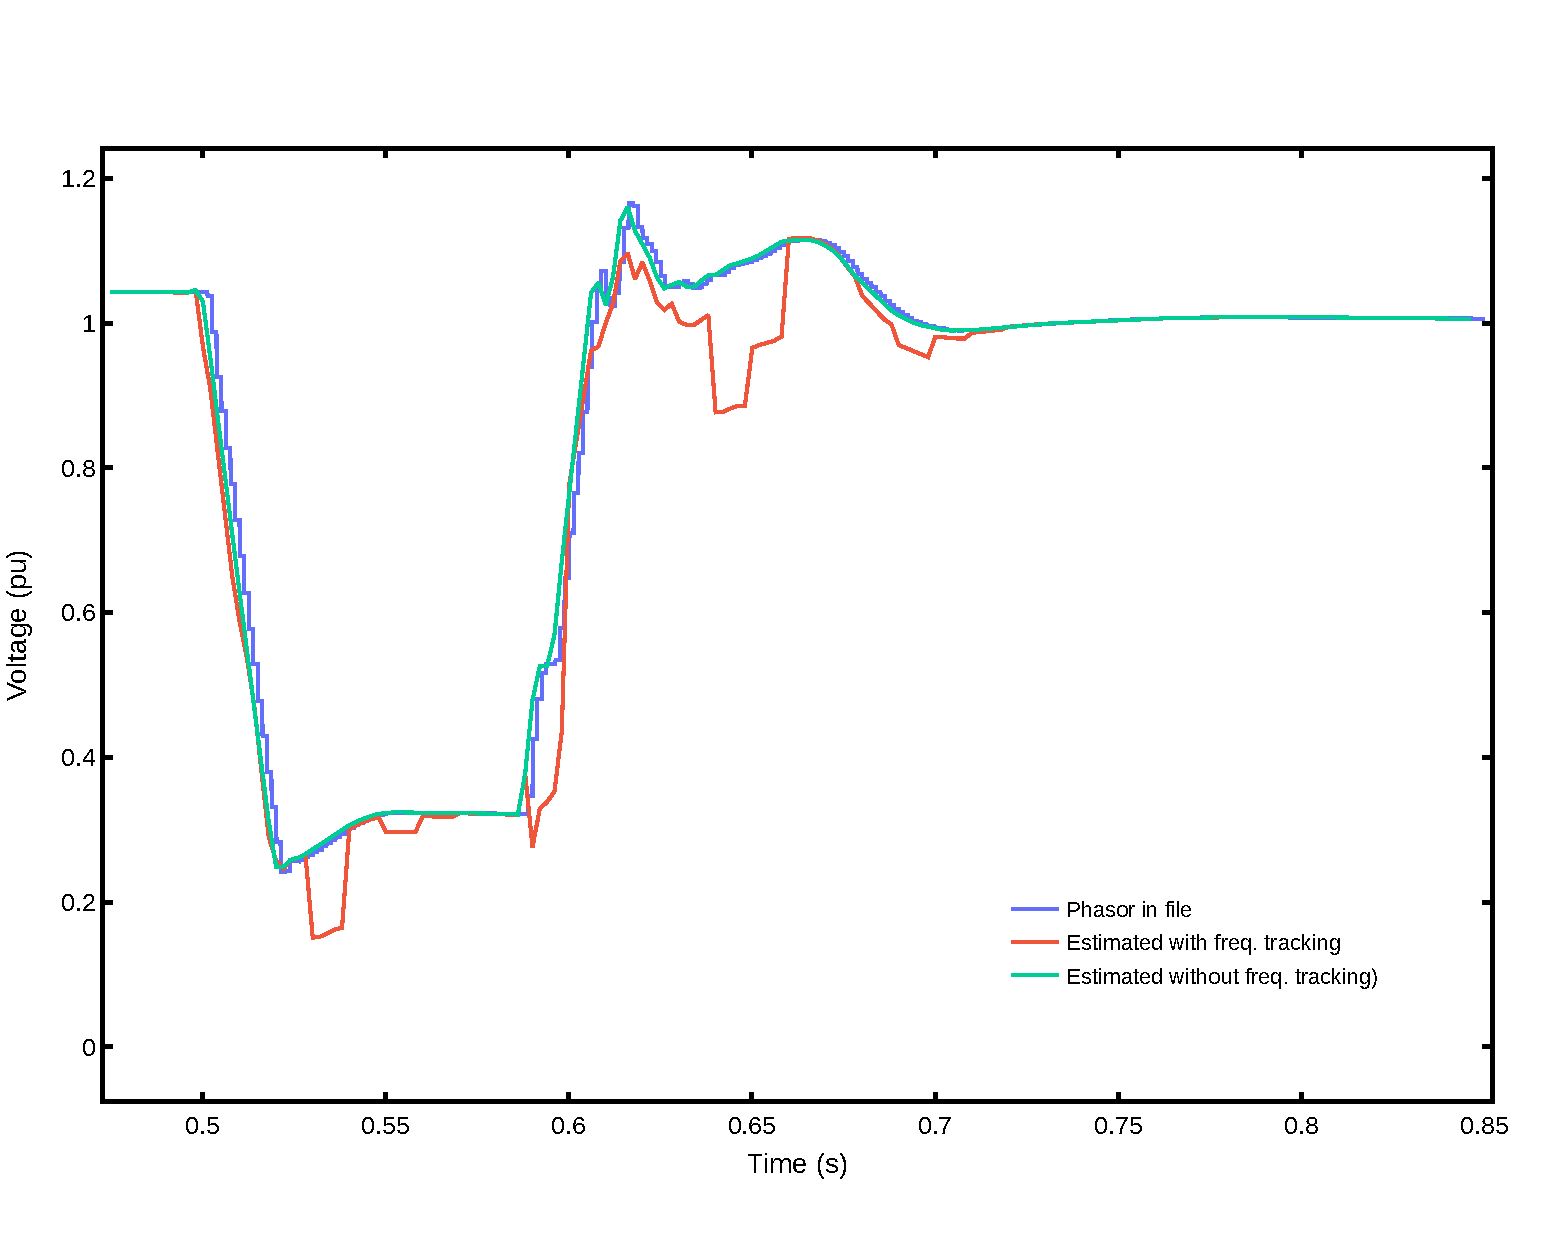
\includegraphics[width=0.48\textwidth]{figs/Fig_emt2rms_exampleV_PS.pdf}
\hfill
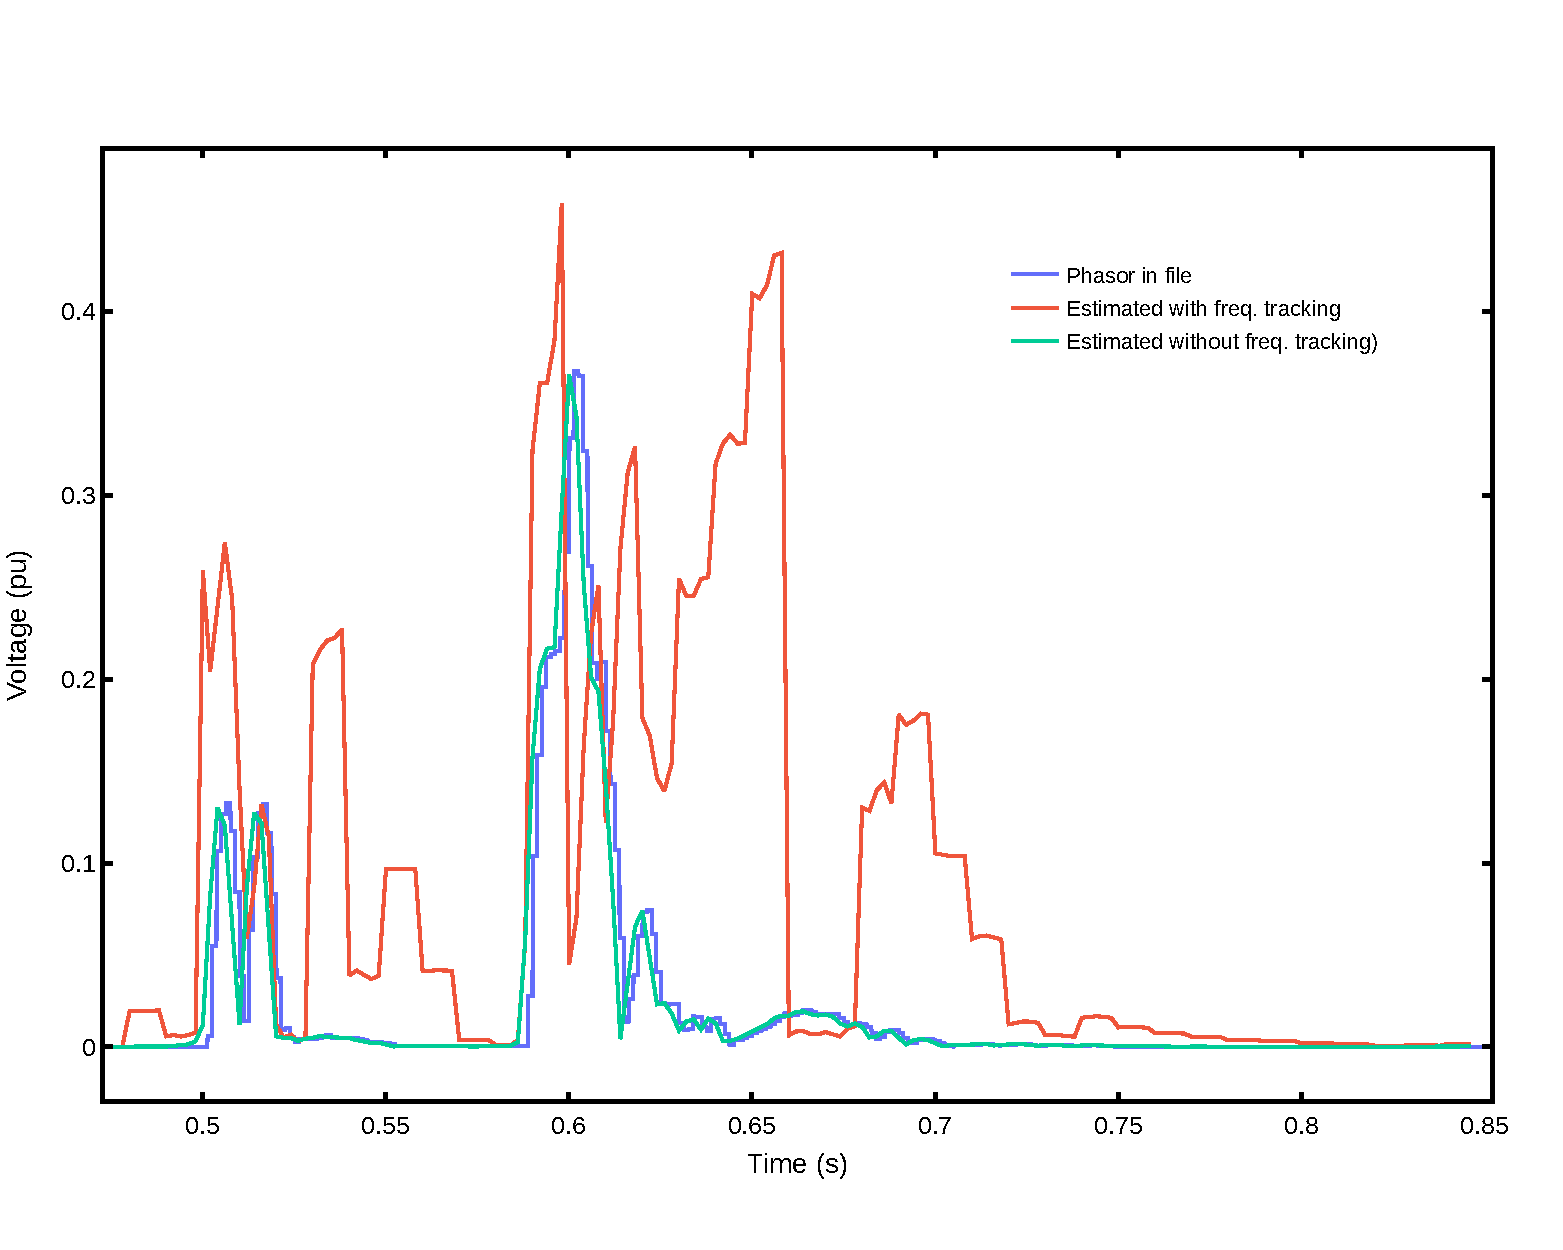
\includegraphics[width=0.48\textwidth]{figs/Fig_emt2rms_exampleV_NS.pdf}
\caption{Conversion of simulated EMT-abc voltages to \ac{rms} \ac{ps}. The
  simulation tool provided its own conversion. For comparison, our own
  conversion with and without frequency tracking. Positive sequence on the left,
  negative sequence on the right.}
\label{fig:emt2rmsV}
\end{figure}

\begin{figure}[t]
\centering
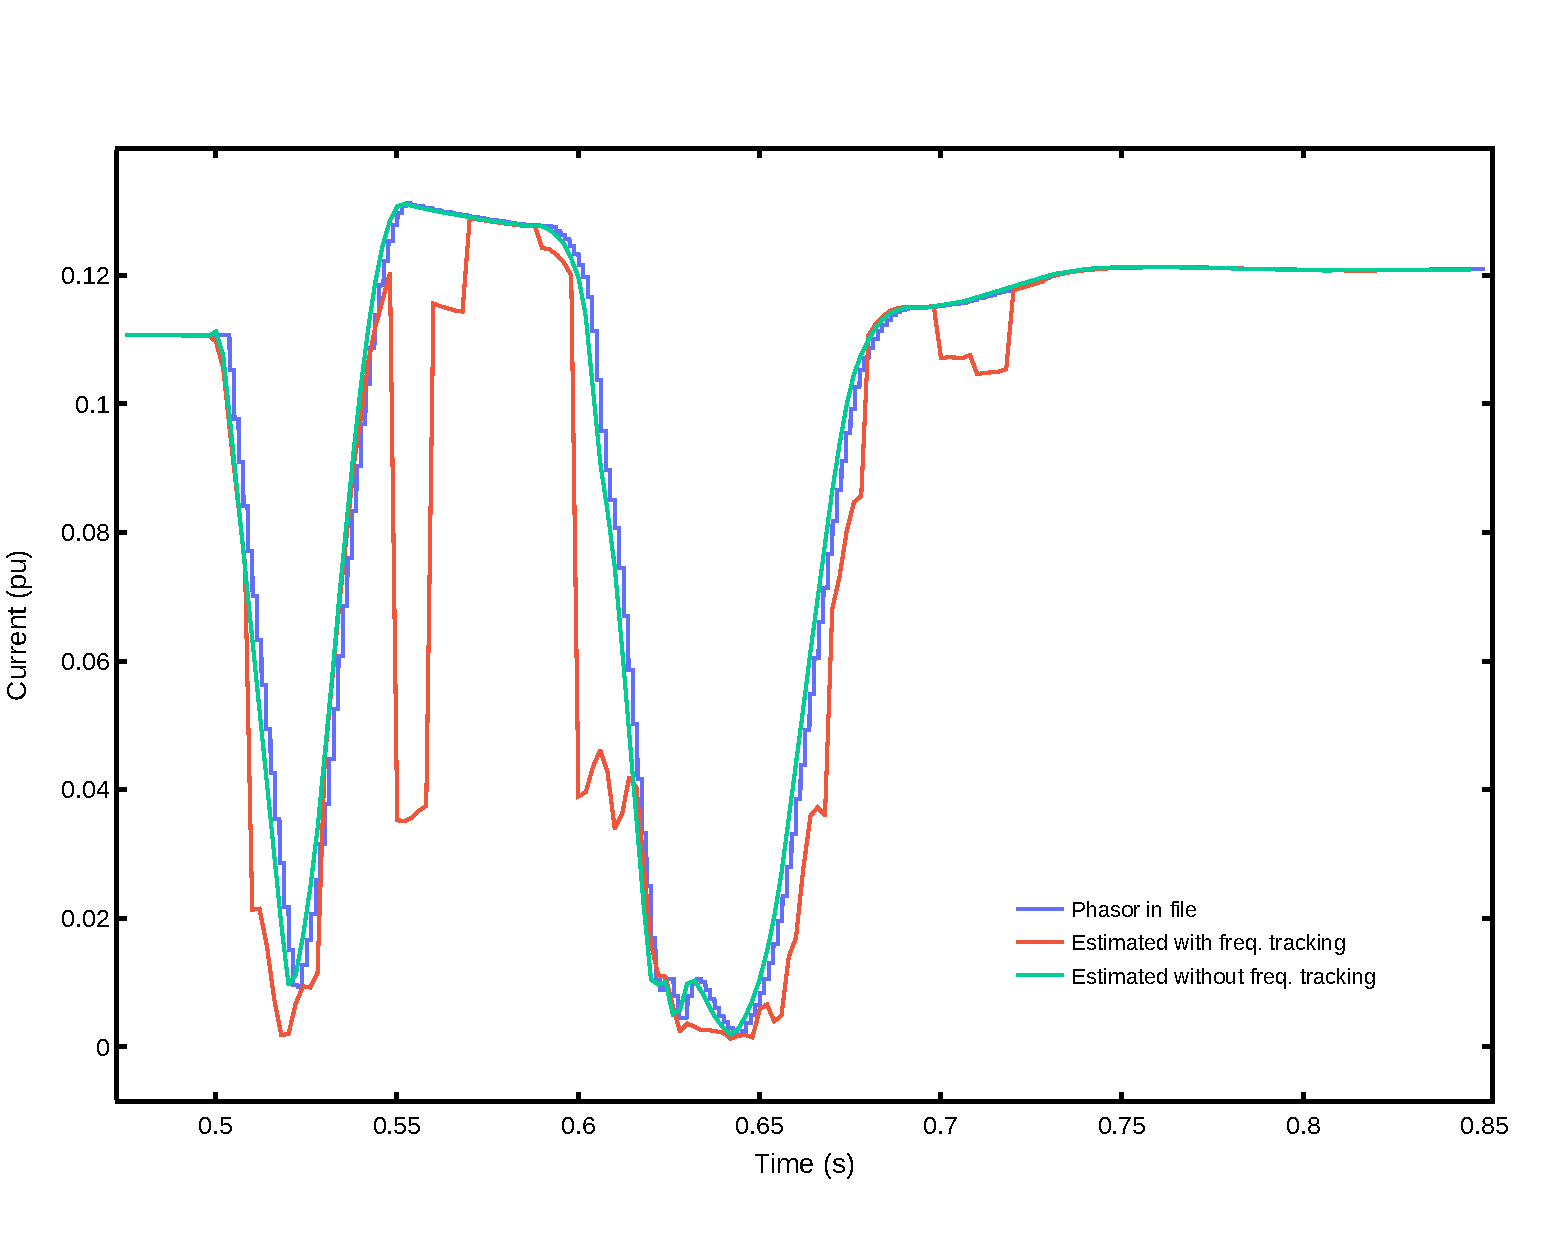
\includegraphics[width=0.48\textwidth]{figs/Fig_emt2rms_exampleI_PS.pdf}
\hfill
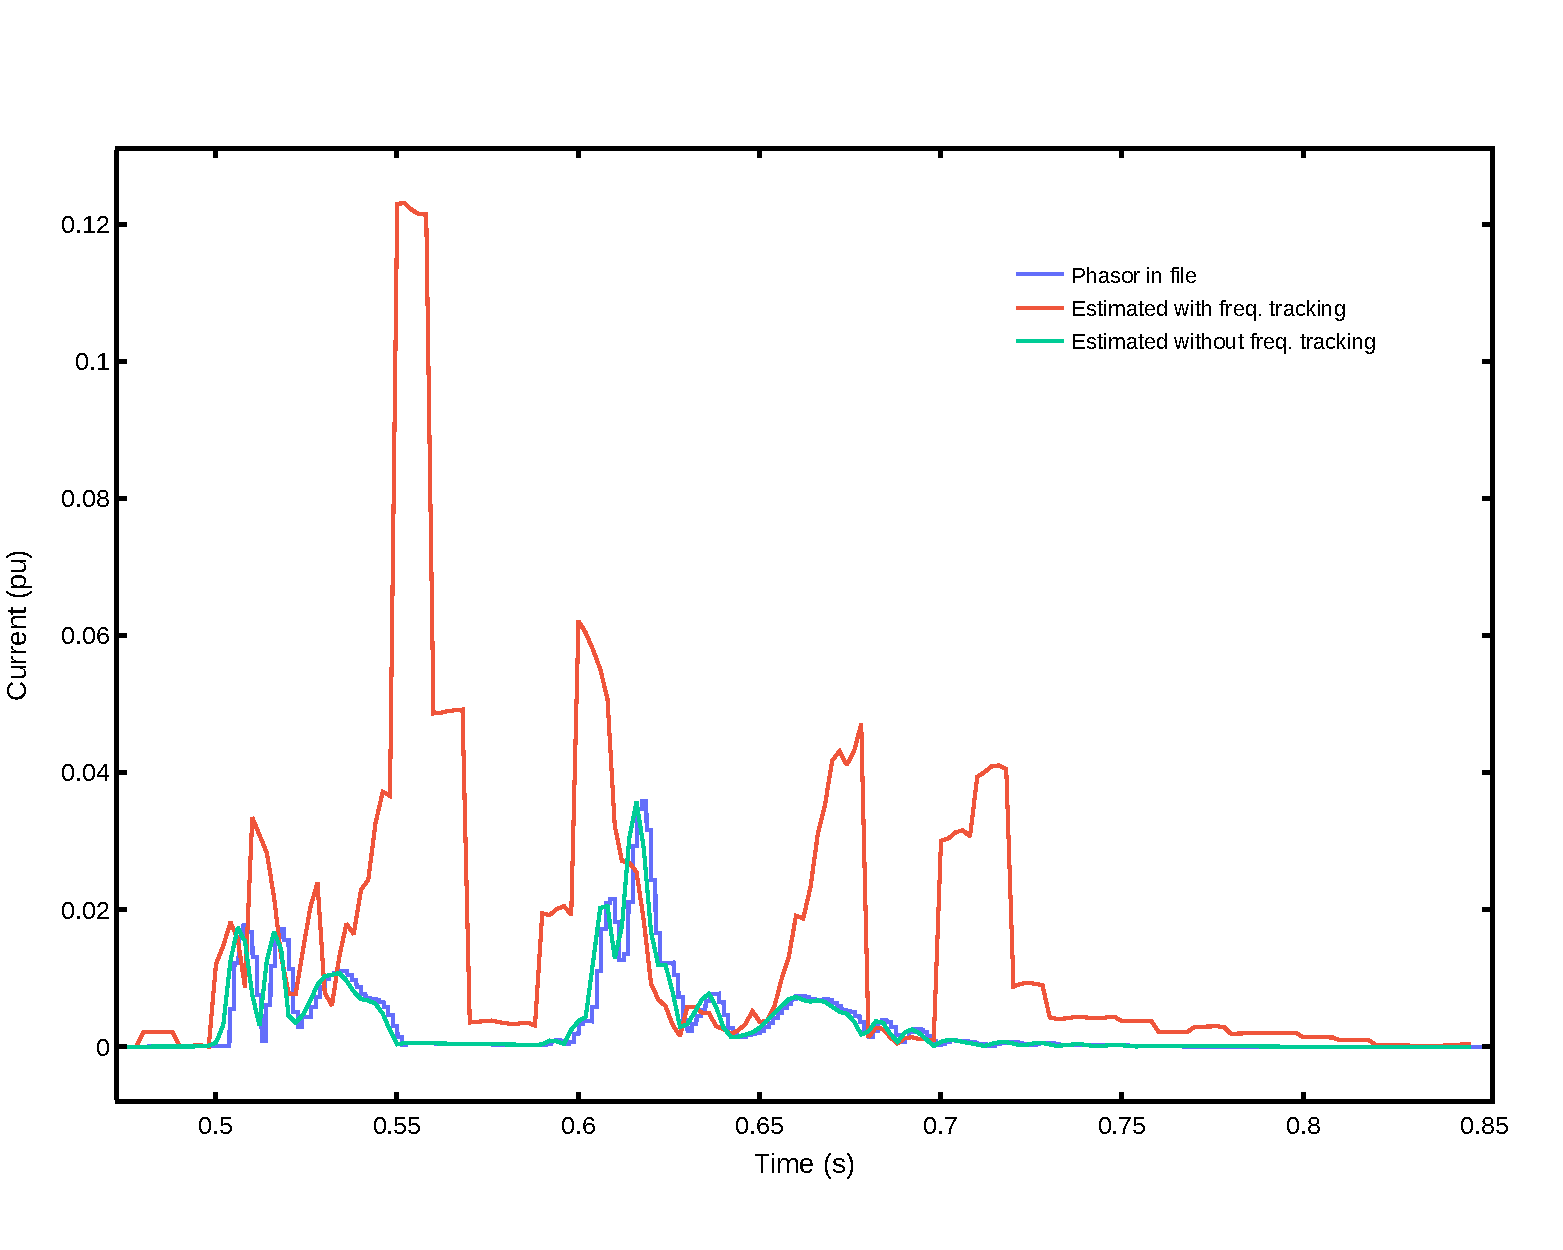
\includegraphics[width=0.48\textwidth]{figs/Fig_emt2rms_exampleI_NS.pdf}
\caption{Same as Fig.~\ref{fig:emt2rmsV}, but for the currents.}
\label{fig:emt2rmsI}
\end{figure}

On the other hand, the sophisticated procedures commonly used in the \ac{dsp}
field are not adequate for this specific purpose. For instance, naive extraction
of the phasor as the peak of the FFT spectrogram closest to the fundamental
frequency (50/60 Hz) is inaccurate, due to the Heisenberg-Gabor
limit~\cite{Smith99}: one cannot obtain high precision for time-domain and
frequency-domain features at the same time (this means that phasor variations
would not have enough time resolution).

In principle, one would think that the most adequate procedures would be those
used in the field of \ac{pmu}, since they exploit the fact that these signals
are \emph{not} arbitrary waves with unknown spectra, but something close to a
sinusoid whose frequency is also quite close to the grid's fundamental--at least
most of the time, i.e., during steady and \emph{quasi-steady} states. This is
actually the key, that the phasor is inherently a steady-state concept and it is
not well defined during fast transients~\cite{PhadkeThorp17}. Therefore, most
phasor estimation algorithms should be supplemented by some kind of
double-check, such as the ``Transient Monitor''~\cite{PhadkeThorp17}
(essentially a check on the signal reconstruction error), in order to flag those
windows where the phasor values are unreliable.

As for the choice of phasor estimation algorithm, a myriad of them exists, each
optimized for different goals.  For instance, the synchrophasor standard
IEC/IEEE 60255-118-1:2018~\cite{pmu-int} describes a reference algorithm for
phasor, frequency, and ROCOF estimation, based on the \ac{dft}. This algorithm
tries to balance the trade-off between three competing aspects of high
importance in \ac{pmu}: (1) immunity to noise, harmonics, off-nominal frequency,
or modulations on the input signal; (2) short reporting latency; and (3) good
time alignment between the phasor, frequency, and ROCOF estimates. For the
purpose of RMS model validation, we can afford to neglect issue (2), and even
(3) when frequency itself is not a signal of interest.

In principle, an algorithm tuned for optimising (1) while preserving high time
resolution would be the most suited solution for offline \ac{emt}-to-\ac{rms}
signal conversion, but it seems to be currently unavailable in the
literature. We therefore tested two methods: a direct implementation of the
procedure described in~\cite{iec27-2}, and a modification of the same in which
one performs dynamic frequency tracking as suggested in the PMU
literature~\cite{PhadkeThorp17,Wang04} (methods based on least squares
regression are potentially more precise, but are out of the scope of this
work). The obtained results are at first counter-intuitive: using no frequency
tracking corrections gives better results. The fact is that, even though adding
dynamic frequency-tracking corrections does achieve more precision (less noise)
in the phasor magnitude \emph{of each abc component}, the phasor angles contain
so much noise that the construction of the symmetrical components becomes very
noisy in the vicinity of transients. By contrast, the phasors extracted with no
frequency tracking exhibit a much cleaner components, as shown in
Fig.~\ref{fig:emt2rmsV} and \ref{fig:emt2rmsI}, even if they are constantly
rotating when the frequency is off-nominal. We compared this calculation against
the conversion produced by a commercial simulation tool, and it seems that the
tool obtains the same result as the no-frequency tracking method proposed in the
standard. The only difference, visible in the figures, was a slight delay (~2ms)
which is probably introduced by some filter.

In any case, one should probably apply the Transient Monitor
technique~\cite{PhadkeThorp17,Wang04} for flagging unreliable phasors, before
ascribing too much credibility to the PS/NS components extracted this way.




\section{Resampling non-uniformly sampled signals to a fixed time-step}
This step usually only applies to RMS signals originated from variable step-size
simulations, but it would also be needed if EMT simulations used a variable
step, or if field data were sampled at irregular intervals (although both cases
are uncommon today). A fixed sampling rate is needed because virtually all
posterior filtering that we may need to apply will use algorithms requiring
uniformly sampled data. While it is clear that this is achieved by some kind of
\emph{interpolation}, the choice of algorithm is not simple, and the IEC
standard is entirely silent on this point.  Moreover, it suggests to resample
both reference and test signals at a common rate at this stage, \emph{before}
low-pass filtering, which may lead to aliasing if the new resampled rate is too
low.  Instead, we advocate to first interpolate the signals independently, then
filter them, and finally downsample both to a common rate, as shown in
Fig.~\ref{fig:RMSModelValidationTool}.

Choosing an adequate method requires the following considerations: the step
sizes are typically very variable, and the signal may contain sharp
discontinuities (jumps of the underlying DAE solver, or even numerical
quantization). Since there is a later stage specifically dedicated to filtering,
we posit that this interpolation stage should strive to be as faithful as
possible to the original signal \emph{in the time domain}. Therefore, our
proposed method is piece-wise polynomial interpolation of the monotone kind,
such as PCHIP (Piecewise Cubic Hermite Interpolating Polynomials). Non-monotone
interpolators, such as cubic splines, would introduce ``ringing'' efects at
sharp transitions, distorting the time-domain curve, as shown in
Fig.~\ref{fig:interp}. Be also aware that packaged routines for resampling may
add their own filtering, which is best to avoid at this stage.  It is true that
piece-wise interpolation may introduce some distortion in the frequency-domain,
at the highest frequencies, but it is better to perform filtering in a dedicated
stage, where one can have full control as described in the next section.

As to the choice of the new sampling rate, in the case of variable step
simulations one should strive to interpolate at the resolution that the
simulator could potentially achieve. This can be guessed from the minimum step
size observed in the data, but it is best if one could have the metadata about
the minimum step size configured for the integrator during the
simulation. Finally, one practical issue: RMS simulators may sometimes output
points at repeated times (typically at point events or sharp changes). One
should remove these before attempting interpolation. Keeping the last repeat is
a good enough strategy, except when the step right before the event is too
long--in which case one should devise a way to separate the time repeats, to
preserve the edge sharpness better.



\section{Low-pass filtering}

At this stage both RMS signals now have a fixed sampled rate (each at its own,
thus preserving their original time resolution). Filtering achieves two goals:
reducing noise in field data (which is mostly high frequency), and smoothing out
high-frequency dynamics to the levels that RMS-model-based simulations can be
trusted to reproduce dynamics with credibility, so that the two signals can be
compared fairly. However, implementing this rough idea into a concrete and
rigorous procedure is not straightforward. The issue is not only the choice of a
cutoff frequency $f_c$ (which the standard sets at 15 Hz), but also the adequacy
of frequency-domain techniques to a problem whose more natural setting is the
time-domain, as we are dealing with transients. Sharp features in transients,
such as those near a fault or a step change, inherently contain
high-frequencies: the Fourier transform of a step function contains harmonics at
all orders $k$, decaying slowly as $1/k$. The DAE solvers in RMS simulations do
indeed output this kind of sharp edges, at time resolutions that can go down to
about 1--5 ms. This means that the ``credible'' bandwidth of RMS simulations may
go up to 100--500Hz. In this light, IEC's $f_c = 15$ Hz proposal seems overly
strict, particularly because of the distorting effect it may have on the
time-domain shape of the rising and falling edges of signal transitions.

Fig.~\ref{fig:filters} shows qualitatively the effects of filtering as one
changes the cutoff frequency $f_c$. The main problem with using a much too low
$f_c$ is that the filter may distort sharp edges too much. This may not be much
of a problem when comparing two signals (MXE, ME, MAE), as long as both are
filtered exactly the same way; however, the values of signal characteristics
such as rise times or overshoot, may be affected. In the case of faults, the IEC
standard proposes the use of exclusion windows right after the fault/clearance
event, to avoid this problem altogether. In the case of other events, this
problem remains.  In the end, the choice of $f_c$ is linked to the fundamental
question: what is the credible time resolution of the underlying RMS models
being used? \textcolor{blue}{You may want to add something here, to conclude
  this discussion}.

%% For this paragraph, see also:
%%   https://electronics.stackexchange.com/questions/14035/whats-the-sharpest-frequency-response-for-a-non-causal-low-pass-filter-whose-st
%%   https://electronics.stackexchange.com/questions/666746/butterworth-filter-damping

On the other hand, the choice of filter \emph{type} is of less importance than
the choice of cut-off frequency, but nevertheless deserves some comments. The
IEC standard rightly prescribes a second-order, critically-damped biquad filter,
but it refrains from explaining the rationale for this choice. The fact is that
this filter has, among second-order filters, the minimum amount of ``ringing''
(i.e., spurious over/undershoot artifacts) at sharp
transitions~\cite{Smith99,Robertson03}; that is, it excels at retaining a sharp
step response. Surely, this filter has poor attenuation of frequencies beyond
the cutoff, but once again we should remind that in this context one wants to
retain \emph{time-domain} fidelity, and frequency-domain considerations are
secondary.  Another valid choice would have been the humble moving average
filter, which is not second-order but it is simpler and even better at
preserving sharp step responses (see Chapter 15 in ~\cite{Smith99}).  The
well-known Bessel filter, which is widely available in packaged routines, is
also a good choice, since is is only slightly underdamped ($\zeta=\sqrt{3}/2$).
Examples of bad choices would be the Butterworth and Chebyshev filters, since
they exhibit ringing in the step response~\cite{Smith99}.


\section{Down-sampling to a common time grid}

It is at this stage that one can downsample the signals to a common rate and not
before, due to the well-known problem of aliasing frequencies.  Both signals are
now sampled at fixed time steps, so one could in principle use any resampling
routine avaiable in DSP packages. However, we advise against this because in
most cases these assume periodic signals; they are based on the FFT and
incorporate aditional filtering.  Instead, and consistent again with the aim of
preserving time-domain features as much as possible, we propose to use monotone
piece-wise interpolation.  The only caution to observe is that, in accordance
with Nyquist's theorem, the new sampling rate should be equal or higher than
$2f_c$ (but lower than the previous rate, of course). Actually, for the sake of
reducing the noise in the MXE/ME/MAE indicators, it is better to use the highest
common rate possible.


\section{Windowing and exclusion zones}

As discussed in the filtering section, the IEC standard addresses the problem of
sharp signal transitions only partially. For fault ride-through tests, it
proposes to compare signals piece-wise in pre/fault/post windows, and to exclude
the instants of time immediately after transitions.  This alleviates the
problems mentioned in the filtering section, but the specific lengths of these
exclusion zones (140 ms after fault, 500 ms after clearance) seem unsuitable
when considering dynamic performance requirements. We think
that... \textcolor{blue}{You may want to add something here. For reference, the
  rationale given by the IEC is: (1) \emph{``The exclusion of the first 140 ms
  of $W_\text{fault}$ from $W_\text{faultQS}$ is mainly due to the limitation of
  the model to replicate the DC-component of the generator flux.''} [...] (2)
  \emph{``The exclusion of the first 500 ms of $W_\text{post}$ from
  $W_\text{postQS}$ is due to the limitation of the model. The accuracy of the
  reactive power is affected by transformer inrush, which could in some cases be
  longer than 500 ms. The accuracy of the active power recovery is affected by
  non-linear aerodynamic effects.''}}





\bibliography{sigproc.bib} 
\bibliographystyle{IEEEtran}

\end{document}

%% EXAMPLE FIG
%% \begin{figure}
%%   \centering
%%   \includegraphics[width=\columnwidth]{figs/myfig}
%%   \caption{Blah...}
%%   \label{fig:blah}
%% \end{figure}

%% EXAMPLE TABLE
%% \begin{table}[!t]
%%   \centering
%%   %% increase table row spacing, adjust to taste
%%   %\renewcommand{\arraystretch}{1.3}
%%   % if using array.sty, it might be a good idea to tweak the value of
%%   % \extrarowheight as needed to properly center the text within the cells
%%   %% Some packages, such as MDW tools, offer better commands for making tables
%%   %% than the plain LaTeX2e tabular which is used here.
%%   \begin{tabular}{lccc}
%%     \hline
%%     \noalign{\smallskip}
%%     Pad\'e order & $\sigma=-0.07-j0.08$ & $-0.14-j0.15$ & $-0.2-j0.22$ \\
%%     & ($|V|=0.92$) & ($|V|=0.81$) &($|V|=0.58$)\\
%%     \noalign{\smallskip}
%%     \hline
%%     \noalign{\smallskip}
%%     [2/2] & 1.795e-03 & 2.30e-02 & 2.74e-01 \\
%%     {}[5/5] & 7.02e-09 & 2.10e-05 & 5.85e-02 \\
%%     {}[10/10] & 0 & 1.89e-10 & 1.16e-02 \\
%%     {}[15/15] & 0 & 1.55e-15 & 2.86e-03 \\
%%     {}[20/20] & 0 & 0 & 7.38e-04 \\
%%     \noalign{\smallskip}
%%     \hline
%%   \end{tabular}
%%   \caption{Examples of relative precision of Pad\'e Approximants vs. order.}
%%   \label{tbl:padecalc}
%% \end{table}
